\chapter{非线性方程和方程组的数值解法}

\begin{definition}
    {非线性方程(组)}{}
    给定(非线性)光滑(smooth)映射$f:\Omega\to\FF^n$,其中$\Omega\subset\FF^n$,寻找$x\in\Omega$满足方程$f(x)=0$,
    称$x$是方程的根(root)。
\end{definition}

% \begin{remark}
%     关心的问题:
%     根的存在性、个数、计算方法。
% \end{remark}

\begin{example}
    {非线性方程的例子}{}
    \begin{itemize}
        \item 代数方程:$p\in\poly_n\subset\cont^\infty(\CC)$
        \[
            p(x)=a_0+a_1x+\cdots+a_nx^n=0,
        \]
        \item 超越方程:如$3x^2-\e x=0$。
    \end{itemize}
\end{example}

\section{非线性方程的不动点迭代法}

迭代法是求解非线性代数方程的重要方法。
其技术路线是将$f(x)=0$的根转化为求解$\varphi(x,\ldots,x)$的不动点(fixed point)。再利用不动点迭代:
\begin{equation}
    x_{i+1}=\varphi(x_i,x_{i-1},\ldots,x_{i-m}),
\end{equation}
特别地,$x_{i+1}=\varphi(x_i)$称为单步方法。
\begin{center}
    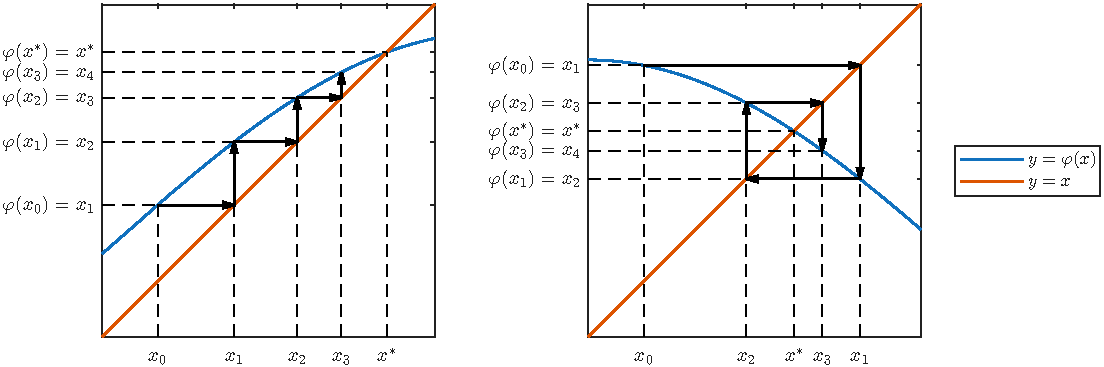
\includegraphics[width=0.95\linewidth]{figures/fixpoint.pdf}
    \captionof{figure}{不动点迭代法示意图}
    \label{fig:fixpoint}
\end{center}

\subsection{迭代法的收敛性}

\begin{theorem}
    {压缩映像原理}{contraction mapping principle}
    若连续函数$\varphi\in\cont[a,b]$满足:
    \begin{itemize}
        \item 像集$\varphi([a,b])\subset[a,b]$;
        \item Lipschitz条件:$\exists L<1$,使得$\forall x_1,x_2\in[a,b]$均有
        \[
            \abs{\varphi(x_2)-\varphi(x_1)}\leq L\abs{x_2-x_1}.
        \]
    \end{itemize}
    则$\forall x_0\in[a,b]$,迭代序列$x_{i+1}=\varphi(x_i)$收敛到唯一的不动点$x^*$。且
    \begin{equation}
            \abs{x_k-x^*}\leq\frac1{1-L}\min\{\abs{x_{k+1}-x_k},L\abs{x_k-x_{k-1}},\ldots,L^k\abs{x_1-x_0}\}.
    \end{equation}
\end{theorem}

\begin{proof}
    不动点的存在性可由$\psi(x)=\varphi(x)-x$的介值定理可得,唯一性由反证法得到。

    对于不等式,由迭代方程$x_{i+1}=\varphi(x_i)$,可得
    \[
        \abs{x_i-x_{i+1}}=\abs{\varphi(x_{i-1})-\varphi(x_i)}\leq L\abs{x_{i-1}-x_i},
    \]
    对$x_i-x_{i+p}$进行裂项可得,
    \[
        \abs{x_i-x_{i+p}}\leq\abs{x_i-x_{i+1}}+\cdots+\abs{x_{i+p-1}-x_{i+p}}\leq(1+L+\cdots+L^{p-1})\abs{x_i-x_{i+1}}.
    \]
    令$p\to\infty$,则$x_{i+p}=x^*$,即得。
\end{proof}

\begin{corollary}
    对于连续函数$\varphi\in\cont^1[a,b]$,将Lipschitz条件换为$\norm{\varphi'}_\infty\leq L<1$,同样可得$\varphi$在$[a,b]$上存在唯一不动点。
\end{corollary}

\begin{remark}
    \thmref{thm:contraction mapping principle} 给出了$\varphi$在区间$[a,b]$上的全局收敛性。但很多情况下全局收敛性并不容易检验。由此引出$x^*$邻域上的局部收敛性概念。
\end{remark}

\begin{definition}
    {局部收敛性}{local convergence}
    若$x^*$是$\varphi$的不动点,且存在$x^*$的邻域$U$,使得$\forall x^{(0)}\in U$,迭代序列$x^{(k+1)}=\varphi(x^{(k)})\in U$且$x^{(k)}\to x^*$,则称$x^*$是局部收敛的(local convergence),$U$为其局部收敛域。
\end{definition}

\begin{corollary}
    若$x^*$为$\varphi$的不动点,$\varphi$在$x^*$某个邻域$U$上连续且$\abs{\varphi'(x^*)}<1$,则$x^*$局部收敛。
\end{corollary}

\begin{definition}
    {收敛阶}{convergence order}
    给定收敛序列$x_n\to x$,若
    \begin{equation}
        0<\liminf_{n\to\infty}\frac{\abs{x_{n+1}-x}}{\abs{x_n-x}^p}\leq\limsup_{n\to\infty}\frac{\abs{x_{n+1}-x}}{\abs{x_n-x}^p}<+\infty,
    \end{equation}
    则称序列$x_n$是$p$阶收敛的,
    特别地,$p=1$称为线性收敛,$p=2$称为平方收敛;

    若下极限可能为0,则称序列$x_n$是至少$p$阶收敛的;若上极限为0,则称序列$x_n$是超$p$阶收敛的。
\end{definition}

\begin{example}
    {}{}
    \begin{itemize}
        \item 调和序列$\{1/n\}$和等比序列$\{a^n\}~(\abs a<1)$线性收敛;
        \item 序列$\{\e{-n^2}\}$超线性收敛,但$\forall\epsilon>0$都不是超$(1+\epsilon)$阶收敛;
        \item 序列$\{\e{-\e n}\}$是e阶收敛的。
    \end{itemize}
\end{example}

\begin{definition}
    {收敛效率}{}
    若序列$\{x_n\}$通过某种算法收敛于$x$,收敛阶为$p$,计算每个$x_n$的计算量为$\theta$ (不依赖于$n$),定义
    \[
        EI:=p^{1/\theta},
    \]
    表示收敛效率,即单位计算量下算法的收敛率。
\end{definition}

\begin{theorem}
    {单步迭代法的收敛阶}{iteration convergence order}
    若$\varphi$在其不动点$x^*$上的一个邻域$U$上足够光滑,则$x_{i+1}=\varphi(x_i)$
    \begin{center}
        在$x^*$处$p$阶局部收敛$\iff\varphi'(x^*)=\cdots=\varphi^{(p-1)}(x^*)=0,\enspace\varphi^{(p)}(x^*)\neq 0$
    \end{center}
\end{theorem}

\begin{proof}
    在$x^*$上作Taylor展开,对于$x_k$,$\exists\xi\in U$介于$x_k,x^*$之间使得
    \[
        \varphi(x_k)=\varphi(x^*)+\varphi'(x^*)(x_k-x^*)+\cdots+\frac{\varphi^{(p-1)}(x^*)}{(p-1)!}(x_k-x^*)^{p-1}+\frac{\varphi^{(p)}(\xi)}{p!}(x_k-x^*)^p,
    \]
    而$\varphi'(x^*)=\cdots=\varphi^{(p-1)}(x^*)=0$,故
    \[
        \frac{x_{k+1}-x^*}{(x_k-x^*)^p}=\frac{\varphi(x_k)-\varphi(x^*)}{(x_k-x^*)^p}
        =\frac{\varphi^{(p)}(\xi)}{p!}\to\frac{\varphi^{(p)}(x^*)}{p!}.
        \qedhere
    \]
    % 由$\varphi^{(p)}$的连续性即得定理结论。
\end{proof}

\subsection{Newton法}

\begin{theorem}
    {Newton迭代法}{Newton's method}
    若$x_k$是$f(x)=0$根$x^*$的一个近似,由Taylor展开,
    \[
        f(x^*)=f(x_k)+f'(x_k)(x^*-x_k)+\bigo(x^*-x_k)^2,
    \]
    若$f'(x_k)\neq 0$,由$f(x^*)=0$,可得 
    \[
        x^*=x_k-\frac{f(x_k)}{f'(x_k)}+\bigo(x^*-x_k)^2,
    \]
    忽略二阶项,剩余项作为$x^*$新的近似$x_{k+1}$,可得Newton迭代法:
    \begin{equation}
        \label{eqn:Newton iter}
        x_{k+1}=x_k-\frac{f(x_k)}{f'(x_k)}.
    \end{equation}
\end{theorem}

\begin{corollary}
    对应迭代函数
    \[
        \varphi(x)=x-\frac{f(x)}{f'(x)},\implies\varphi'(x)=\frac{f(x)f''(x)}{f'(x)^2},
    \]
    故$\varphi'(x^*)=0$,Newton迭代法是超线性收敛的。
\end{corollary}

\begin{remark}
    Newton法的几何解释:$f$在$x_k$处的切线
    \[
        y=f(x_k)+f'(x_k)(x-x_k),
    \]
    与$x$轴的交点作为$x^*$新的近似$x_{k+1}$。
\end{remark}

\begin{theorem}
    {Newton迭代法的局部收敛性}{convergence of Newton's method}
    若根$x^*$处导数$f'(x^*)\neq 0$且$f''$在$x^*$邻域$U$上连续,则Newton法至少二阶收敛。
\end{theorem}

\begin{proof}
    由Taylor展开,$\exists\xi\in U$介于$x^*,x_k$之间使得
    \[
        f(x^*)=f(x_k)+f'(x_k)(x^*-x_k)+\frac{f''(\xi)}2(x^*-x_k)^2,
    \]
    而$f(x^*)=0$,故
    \[
        \frac{x_{k+1}-x^*}{(x_k-x^*)^2}=\frac{f''(\xi)}{2f'(x_k)}\to\frac{f''(x^*)}{2f'(x^*)}.
    \]
    故Newton法至少二阶收敛;当$f''(x^*)\neq 0$时,Newton法就是二阶收敛的。
\end{proof}

\begin{remark}
    Newton法至少二阶收敛的前提之一是$f'(x^*)\neq 0$,这相当于说$x^*$是$f$的单重根。
\end{remark}

\begin{definition}
    {$r$ - 重根}{multiple root}
    若
    \[
        f(x^*)=f'(x^*)=\cdots=f^{(r-1)}(x^*)=0,\enspace f^{(r)}(x^*)\neq 0,
    \]
    则称$x^*$是$f$的一个$r$ - 重根(multiple root)。
\end{definition}

\begin{corollary}
    若$x^*$是$f$的$r$ - 重根,则$\exists\xi,\eta$介于$x_k,x^*$之间使得,
    \[
        \varphi(x_k)=x_k-\frac{f(x^*)+f'(x^*)(x_k-x^*)+\cdots+f^{(r)}(\xi)(x-x^*)^r/r!}{f'(x^*)+f''(x^*)(x_k-x^*)+\cdots+f^{(r)}(\xi)(x-x^*)^r/(r-1)!},
    \]
    故
    \[
        \frac{x_{k+1}-x^*}{x_k-x^*}=1-\frac1r\frac{f^{(r)}(\xi)}{f^{(r)}(\eta)}\to1-\frac1r\geq\frac12.
    \]
    Newton法变为线性收敛的!故需要对Newton法进行改进。
\end{corollary}

\begin{theorem}
    {Newton法的改进}{}
    若$x^*$为$f$的$r$ - 重根,则依前文推论将Newton法\eqref{eqn:Newton iter}改进为二阶收敛的: 
    \begin{equation}
        \label{eqn:Newton iter r-multiroot}
        x_{k+1}=x_k-r\frac{f(x_k)}{f'(x_k)},
    \end{equation}
    \tcblower
    对
    \begin{equation}
        u(x):=\frac{f(x)}{f'(x)},
    \end{equation}
    使用Newton法\eqref{eqn:Newton iter},
    易于验证,$x^*$是$u$的单重根。
\end{theorem}

\subsection{割线法}

下面再介绍一种多步迭代方法。

\begin{theorem}
    {割线法}{secant method}
    以$f$在$x_k,x_{k-1}$的割线斜率(差商)
    \[
        f[x_k,x_{k-1}]=\frac{f(x_k)-f(x_{k-1})}{x_k-x_{k-1}}
    \]
    代替Newton法\eqref{eqn:Newton iter}中的导数$f'(x_k)$,称为割线法(secant method):
    \begin{equation}
        \label{eqn:secant line}
        x_{k+1}=x_k-\frac{x_k-x_{k-1}}{f(x_k)-f(x_{k-1})}f(x_k),
    \end{equation}
\end{theorem}

\begin{theorem}
    {割线法的收敛性}{}
    若在根$x^*$的邻域$U(x^*,\delta)=[x^*-\delta,x^*+\delta]$上$f'(x)\neq 0$且$f\in\cont^2(U)$,若
    \[
        M=\frac{\max_{x\in U}\abs{f''(x)}}{2\min_{x\in U}\abs{f'(x)}}<+\infty,
    \]
    则给定$x_0,x_1\in U(x^*,\min(\delta,1/M))$,割线法$(1+\phi)$阶收敛到$x^*$。
\end{theorem}

\begin{proof}
    记$e_k=x_k-x^*$,则 
    \[
        e_{k+1}=e_k-\frac{f(x_i)-f(x^*)}{f[x_k,f_{k-1}]}=e_k\frac{f[x_k,x_{k-1}]-f[x_k,x^*]}{f[x_k,x_{k-1}]},
    \]
    故$\exists\xi,\eta\in U$使得
    \[
        e_{k+1}=e_ke_{k-1}\frac{f[x_k,x_{k-1},x^*]}{f[x_k,x_{k-1}]}=e_ke_{k-1}\frac{f''(\xi)}{2f'(\eta)},
    \]
    故
    \[
        \abs{e_{k+1}}\leq\abs{e_k}\abs{e_{k-1}}M\leq\abs{e_k}M\min(\delta,1/M)
    \]
    由于$e_k$至少线性收敛,故 % $\forall\epsilon>0$,$\exists N>0$足够大使得$\forall k>N$,有
    \[
        \abs{e_{k+1}}\approx\abs{e_k}\abs{e_{k-1}}M^*,\quad M^*=\frac{\abs{f''(x^*)}}{2\abs{f'(x^*)}},
    \]
    其中$a_n\approx b_n$表示$\lim_{n\to\infty}a_n-b_n=0$。对上式取对数得到
    \[
        \ln(M^*\abs{e_{k+1}})\approx\ln(M^*\abs{e_k})+\ln(M^*\abs{e_{k-1}}),
    \]
    当$k\to\infty$时,上式变为等号,符合Fibonacci数列递推式,故阶数为$1+\phi=\frac{1+\sqrt5}2$。
\end{proof}

\begin{remark}
    Newton法与割线法比较:
    \begin{itemize}
        \item 割线法不用求导;
        \item 当$x_k$接近$x^*$时舍入误差对割线法影响较大;
        \item 割线法的效率$EI_1=1+\phi$;Newton法的效率$EI_2=2^{1/\theta}$,其中$\theta$是计算$f'(x)$相对差分的计算量。当
        \[
            \theta>\frac1{\log_2(1+\phi)}>1.44
        \]
        时,割线法效率更高。
    \end{itemize}
\end{remark}

\subsection{Aitken加速方法}

由\thmref{thm:iteration convergence order},若$\abs{\varphi'(x^*)}\in(0,1)$,则迭代收敛速度为线性的。由于
\[
    x_{k+2}-x^*=\varphi'(\xi)(x_{k+1}-x^*)\approx\varphi'(x^*)(x_{k+1}-x^*),
\]
下一项$x_{k+1}-x^*\approx\varphi'(x^*)(x_k-x^*)$,故可联立消掉$\varphi'(x^*)$,得到:
\begin{equation}
    x^*\approx x_k-\frac{(x_{k+1}-x_k)^2}{x_{k+2}-2x_{k+1}+x_k}\equiv x_k-\frac{\D x_k^2}{\D^2 x_k}.
\end{equation}
其中差分$\D x_k=x_{k+1}-x_k$,二阶差分$\D^2x_k=\D x_{k+1}-\D x_k$。和微分记号一样,约定$\D x_k^2\equiv(\D x_k)^2$,而$\D(x_k^2)$需要加括号。

\begin{theorem}
    {Aitken加速方法}{Aitken}
    若$x_k$至少线性收敛到$x^*$,则可定义
    \begin{equation}
        \label{eqn:Aitken}
        x_k':=x_k-\frac{\D x_k^2}{\D^2x_k},
    \end{equation}
    并且$x_k'$收敛比$x_k$快:
    \[
        \lim_{k\to\infty}\frac{x_k'-x^*}{x_k-x^*}=0.
    \]
\end{theorem}

\begin{proof}
    记$e_k:=x_k-x^*$,由$x_k$至少线性收敛,$\exists\lambda$且$\abs\lambda<1$使得 
    \[
        e_{k+1}=(\lambda+\delta_k)e_k,\quad\delta_k\to 0.
    \]
    则
    \begin{align*}
        \D x_k&=e_{k+1}-e_k=e_k[(\lambda-1)+\delta_k],\\
        \D^2x_k&=e_{k+2}-2e_{k+1}+e_k=e_k[(\lambda+\delta_{k+1})(\lambda+\delta_k)-2(\lambda+\delta_k)+1]=e_k[(\lambda-1)^2+\mu_k],
    \end{align*}
    其中$\mu_k=\lambda(\delta_{k+1}+\delta_k)-2\delta_k+\delta_k\delta_{k+1}\to 0$。当$k$充分大时,$\D^2x_k\neq 0$,可定义$x_k'$,且
    \[
        \lim_{k\to\infty}\frac{x_k'-x^*}{x_k-x^*}=\lim_{k\to\infty}1-\frac{[(\lambda-1)+\delta_k]^2}{(\lambda-1)^2+\mu_k}=0.
        \qedhere
    \]
\end{proof}

\begin{remark}
    Aitken加速方法只需给定序列$x_k$,其公式\eqref{eqn:Aitken}与序列$x_k$的产生方法$\varphi$无关。
\end{remark}

\subsection{Steffensen迭代法}

\begin{theorem}
    {Steffensen迭代法}{Steffensen}
    对Aitken加速公式\eqref{eqn:Aitken}利用$x_{k+1}=\varphi(x_k),\,x_{k+2}=\varphi(\varphi(x_k))$作为新的迭代公式:
    \[
        \hat x_{k+1}=\hat x_k-\frac{(\varphi(\hat x_k)-\hat x_k)^2}{\varphi(\varphi(\hat x_k))-2\varphi(\hat x_k)+\hat x_k}.
    \]
    这实际上根据$\varphi$定义了新的迭代函数
    \begin{equation}
        \psi(x)=x-\frac{(\varphi(x)-x)^2}{\varphi(\varphi(x))-2\varphi(x)+x}=\frac{x\varphi(\varphi(x))-\varphi(x)^2}{\varphi(\varphi(x))-2\varphi(x)+x}.
    \end{equation}
    若$x^*$是$\psi$的不动点,则$x^*$也是$\varphi$的不动点;

    若$x^*$是$\varphi$的不动点,$\varphi\in\cont^1(U)$且$\varphi'(x^*)\neq 1$,则$x^*$是$\psi$的不动点。
\end{theorem}

\begin{proof}
    由$\psi$表达式可得,
    % \[
    %     (x-\psi(x))(\varphi(\varphi(x))-2\varphi(x)+x)=(\varphi(x)-x)^2,
    % \]
    $\psi(x^*)=x^*\implies\varphi(x^*)=x^*$;
    而$\varphi(x^*)=x^*$时,$\psi(x^*)$出现0/0型,由L'H\^opital法则
    \[
        \psi(x^*)=x^*-\lim_{x\to x^*}\frac{(\varphi(x)-x)^2}{\varphi(\varphi(x))-2\varphi(x)+x}=x^*-\frac{2(\varphi(x^*)-x^*)(\varphi'(x^*)-1)}{\varphi'(\varphi(x^*))\varphi'(x^*)-2\varphi'(x^*)+1}=x^*.
        % \frac{\varphi(\varphi(x^*))+x^*\varphi'(\varphi(x^*))\varphi'(x^*)-2\varphi(x^*)\varphi'(x^*)}{\varphi'(\varphi(x^*))\varphi'(x^*)-2\varphi'(x^*)+1}=x^*.
        \qedhere
    \]
\end{proof}

\begin{remark}
    证明中分母出现了$\varphi'(x^*)-1$,故要求$\varphi'(x_k)\neq 1$,即$x^*$不是$\varphi(x)-x=0$的重根。
    但事实上$\varphi'(x^*)=1$也可以证明$\psi(x^*)=x^*$。
\end{remark}

\begin{theorem}
    {Steffensen迭代法的收敛阶}{convergence order Steffensen}
    若$x_{k+1}=\varphi(x_k)$是$p$阶收敛的($p>1)$,则$x_{k+1}=\psi(x_k)$是$(2p-1)$阶收敛的。

    若$p=1$且$\varphi'(x^*)\neq 1$,则$x_{k+1}=\psi(x_k)$是二阶收敛的。
\end{theorem}

\begin{proof}
    由$\varphi$是$p$阶收敛的:$\varphi(x)-x^*=\Theta(x-x^*)^p,\;\varphi(\varphi(x))-x^*=\Theta(x-x^*)^{2p}$,
    \begin{align*}
        \psi(x)-x^*&=\frac{(x-x^*)(\varphi(\varphi(x))-x^*)-(\varphi(x)-x^*)^2}{\varphi(\varphi(x))-x^*-2(\varphi(x)-x^*)+x-x^*}\\
        &=\frac{\Theta(x-x^*)^{2p+1}-\Theta(x-x^*)^{2p}}{\Theta(x-x^*)^{2p}-\Theta(x-x^*)^p+x-x^*}=\Theta(x-x^*)^{2p-1}.
        \qedhere
    \end{align*}
\end{proof}

\begin{remark}
    若$\varphi\in\cont^2(U)$且$\varphi'(x^*)\neq 1$,则Steffensen法不但可以提高收敛速度(至少二阶收敛),在$\abs{\varphi'(x^*)}>1$时还可以把不收敛的方法改进为二阶收敛的方法。
    但当$p>1$时,Steffensen法一般好处不大,故其多用于改进线性收敛的情形。
\end{remark}

\begin{example}
    {}{}
    特别地,$\varphi(x)=x+f(x)$,
    % 则$\varphi(\varphi(x))=\varphi(x+f(x))=x+f(x)+f(x+f(x))$
    可得
    \begin{equation}
        \psi(x)=x-\frac{f(x)^2}{f(x+f(x))-f(x)}.
    \end{equation}
    若$f(x^*)=0$,可得$\psi(x^*)=x^*,\;\psi'(x^*)=0$故$x_{k+1}=\psi(x_k)$至少二阶收敛。
\end{example}

\section{非线性方程组的不动点迭代法}

\begin{definition}
    {向量值函数}{vector function}
    向量值函数是一个映射$F:D\to\RR^n$,其中$D\subset\RR^n$,其分量是多元标量函数$f_i:D\to\RR$:
    \begin{equation}
        F(x)=\begin{bmatrix}
            f_1(x_1,\ldots,x_n)\\\vdots\\f_m(x_1,\ldots,x_n)
        \end{bmatrix}
    \end{equation}
\end{definition}

\begin{definition}
    {向量值函数的连续性}{vector function continuous}
    给定点$x_0\in D$,若$\forall\epsilon>0,\;\exists\delta>0$使得领域内$\forall x\in B(x_0,\delta)\subset D$均有
    \[
        \norm{F(x)-F(x_0)}<\epsilon,
    \]
    则称$F$在$x_0$处连续。
\end{definition}

\begin{definition}
    {向量值函数的导数}{}
    给定$x\in D$和充分小$h$使得$x+h\in D$,若存在矩阵$A(x)\in\RR^{m\times n}$满足 
    \begin{equation}
        \lim_{h\to 0}\frac{\norm{F(x+h)-F(x)-A(x)h}}{\norm h}=0,
    \end{equation}
    则称$F$在$x$处可微,$A(x)=:F'(x)$称为$F$的导数,事实上就是Jacobi矩阵:
    \begin{equation}
        F'(x)=\begin{bmatrix}
            \pv{f_1}{x_1}&\cdots&\pv{f_1}{x_n}\\
            \vdots&\ddots&\vdots\\
            \pv{f_m}{x_1}&\cdots&\pv{f_m}{x_n}
        \end{bmatrix}
    \end{equation}
\end{definition}

\begin{theorem}
    {压缩映像原理(向量形式)}{contraction mapping principle (vector)}
    连续函数$\varphi:D\subset\RR^n\to\RR^n$满足:
    \begin{itemize}
        \item 闭性:$D$是闭集;
        \item 映内性:$\varphi(D)\subset D$;
        \item 压缩性:$\exists L<1$,使得$\forall x_1,x_2\in D$,
        \[
            \norm{\varphi(x_2)-\varphi(x_1)}\leq L\norm{x_2-x_1},
        \]
    \end{itemize}
    则$\forall x_0\in D$,迭代序列$x_{k+1}=\varphi(x_k)$收敛到$\varphi$唯一的不动点$x^*$。
\end{theorem}

\begin{remark}
    压缩性依赖于范数的选择。如$\varphi(x)=Ax$,其中
    \[
        \varphi'(x)=A=\begin{bmatrix}
            0.1&0.9\\0&0.1
        \end{bmatrix}.
    \]
    在2 - 范数下$\norm A_2<1$可压缩,但在无穷范数下$\norm A_\infty=1$不可压缩。
\end{remark}

\begin{definition}
    {局部收敛性(向量形式)}{}
    给定$\varphi(x^*)$的不动点,若存在$x^*$的一个邻域$S\subset D$使得$\forall x^{(0)}\in S$,$x^{(k+1)}=\varphi(x^{(k)})\in S$且$x^{(k)}\to x^*$,则称$x^*$是局部收敛的。
\end{definition}

\begin{theorem}
    {}{}
    若$\exists L\in(0,1)$和某个范数$\norm\cdot$使得$\forall x\in S(x^*,\delta)$均有
    \[
        \norm{\varphi(x)-\varphi(x^*)}\leq L\norm{x-x^*},
    \]
    则$x^*$是局部收敛的。
\end{theorem}

\begin{corollary}
    一个充分条件:若存在一个算子范数使得$\norm{\varphi'(x^*)}<1$,则$x^*$是局部收敛的。
\end{corollary}

\begin{theorem}
    {Newton法(向量形式)}{}
    给定$x^{(0)}$,计算 
    \[
        x^{(k+1)}=x^{(k)}-F'(x^{(k)})\iv F(x^{(k)}).
    \]
\end{theorem}

\begin{remark}
    Newton法的一个显著缺点是需要反复计算$F'$。可借鉴割线法改进。
\end{remark}

\begin{theorem}
    {修正的Newton法}{}
    将Jacobi矩阵$F'(x^{(k)})$替换为矩阵$A^{(k)}$:
    \[
        x^{(k+1)}=x^{(k)}-{A^{(k)}}\iv F(x^{(k)}),
    \]
    矩阵$A^{(k)}$满足拟Newton方程:
    \begin{equation}
        A^{(k)}(x^{(k)}-x^{(k-1)})=F(x^{(k)})-F(x^{(k-1)}),
    \end{equation}
    显然$A^{(k)}$的取法并不唯一,可以迭代地写成
    \[
        A^{(k+1)}=A^{(k)}+\D A^{(k)},
    \]
    且$\rank(A^{(k)})$一般为1或2,即$A^{(k+1)}$是$A^{(k)}$的一个低秩修正。
\end{theorem}

\begin{theorem}
    {Broyden秩1方法}{}
    令$p^{(k)}=x^{(k+1)}-x^{(k)},\;q^{(k)}=F(x^{(k+1)})-F(x^{(k)})$,设$\D A^{(k)}=u^{(k)}{v^{(k)}}\tp$是秩1矩阵,则
    \[
        (A^{(k)}+u^{(k)}{v^{(k)}}\tp)p^{(k)}=q^{(k)},\implies u^{(k)}=\frac{q^{(k)}-A^{(k)}p^{(k)}}{{v^{(k)}}\tp p^{(k)}},
    \]
    可令$v^{(k)}=p^{(k)}$,则 
    \begin{subequations}
        \begin{align}
            x^{(k+1)}&=x^{(k)}-{A^{(k)}}\iv F(x^{(k)}),\\
            \D A^{(k)}&=\frac{(q^{(k)}-A^{(k)}p^{(k)}){p^{(k)}}\tp}{\norm{p^{(k)}}^2},\\
            A^{(k+1)}&=A^{(k)}+\D A^{(k)}.
        \end{align}
    \end{subequations}
\end{theorem}
